%%%%%%%%%%%%%%%%%%%%%%%%%%%%%%%%%%%%%%%%%%%%%%%%%%%%%%%%%%%%%%%%%%%%%%%%%%%%%%%%
%%%%%%%%%%%%%%%%%%%%%%%%%%%%%%%%%%%%%%%%%%%%%%%%%%%%%%%%%%%%%%%%%%%%%%%%%%%%%%%%
%%%%%%%%%%%%%%%%%%%%%%%%%%%%%%%%%%%%%%%%%%%%%%%%%%%%%%%%%%%%%%%%%%%%%%%%%%%%%%%%
%%%%%%%%%%%%%%%%%%%%%%%%%%%%%%%%%%%%%%%%%%%%%%%%%%%%%%%%%%%%%%%%%%%%%%%%%%%%%%%%
\chapter{Pierre-Simon de Laplace\label{annexe-lap_irl}}
%%%%%%%%%%%%%%%%%%%%%%%%%%%%%%%%%%%%%%%%%%%%%%%%%%%%%%%%%%%%%%%%%%%%%%%%%%%%%%%%
%%%%%%%%%%%%%%%%%%%%%%%%%%%%%%%%%%%%%%%%%%%%%%%%%%%%%%%%%%%%%%%%%%%%%%%%%%%%%%%%
%%%%%%%%%%%%%%%%%%%%%%%%%%%%%%%%%%%%%%%%%%%%%%%%%%%%%%%%%%%%%%%%%%%%%%%%%%%%%%%%
%%%%%%%%%%%%%%%%%%%%%%%%%%%%%%%%%%%%%%%%%%%%%%%%%%%%%%%%%%%%%%%%%%%%%%%%%%%%%%%%
\chaptermark{Pierre-Simon de Laplace}
%-------------------------------------------------------------------------------
\begin{marginfigure}
    \centering
    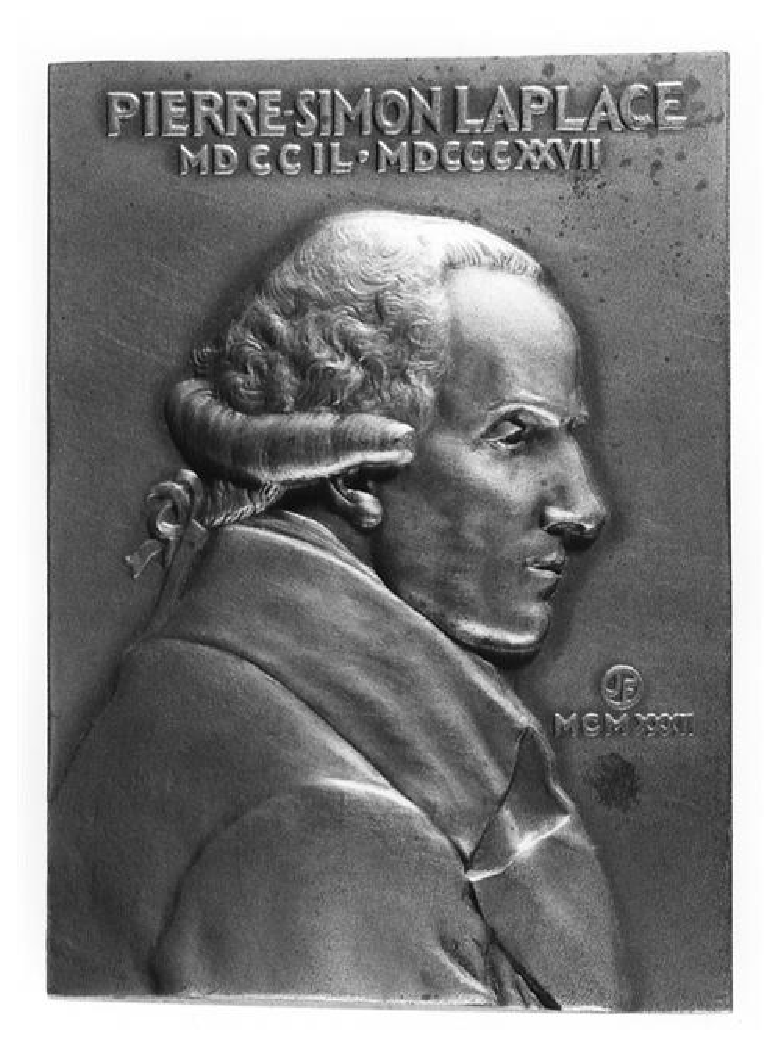
\includegraphics[width=0.9\linewidth]{fig/Pierre-Simon-Laplace_2}
    \captionsetup{width=0.8\linewidth}
    \caption*{Pierre-Simon, marquis de Laplace,  (1745-1827) mathématicien 
             et astronome français. (Paris, musée d'Orsay)}
\end{marginfigure}
%-------------------------------------------------------------------------------
\indent Pierre-Simon de Laplace, né Pierre-Simon Laplace, comte Laplace, puis 
1er marquis de Laplace, né le 23 mars 1749 à Beaumont-en-Auge et mort le 5 
mars 1827 à Paris, est un mathématicien, astronome, physicien et homme 
politique français.

Laplace est l'un des principaux scientifiques de la période napoléonienne. 
En effet, il a apporté des contributions fondamentales dans différents champs 
des mathématiques, de l'astronomie et de la théorie des probabilités. Il a 
été l'un des scientifiques les plus influents de son temps, notamment par son 
affirmation du déterminisme. Il a contribué de façon décisive à l'émergence 
de l'astronomie mathématique, reprenant et étendant le travail de ses 
prédécesseurs dans son Traité de Mécanique céleste (1799-1825). Cet ouvrage 
majeur, en cinq volumes, a transformé l'approche géométrique de la mécanique
développée par Newton en une approche fondée sur l'analyse mathématique.
%%%%%%%%%%%%%%%%%%%%%%%%%%%%%%%%%%%%%%%%%%%%%%%%%%%%%%%%%%%%%%%%%%%%%%%%%%%%%%%%
%%%%%%%%%%%%%%%%%%%%%%%%%%%%%%%%%%%%%%%%%%%%%%%%%%%%%%%%%%%%%%%%%%%%%%%%%%%%%%%%
%%%%%%%%%%%%%%%%%%%%%%%%%%%%%%%%%%%%%%%%%%%%%%%%%%%%%%%%%%%%%%%%%%%%%%%%%%%%%%%%
%%%%%%%%%%%%%%%%%%%%%%%%%%%%%%%%%%%%%%%%%%%%%%%%%%%%%%%%%%%%%%%%%%%%%%%%%%%%%%%%
%annexe_laplace_irl.tex
